\chapter[INTRODUCTION AND LITERATURE REVIEW]{INTRODUCTION AND \\  LITERATURE REVIEW}

\section{Author's Message}

Howdy! This is my honor to organize the \LaTeX ~ Thesis Template for Texas $A\&M$ University\footnote{This is a test to see how the footnote is display in long long text below the main content. The font size is 10pt if you doesn't modify the default setting. As you can see, it is single space.} as a graduate student at ECE under the guidance of OGAPS@TAMU. I have been applied \LaTeX~ to write my bachelor and master thesis in Chinese and English previously. My approach is to deal with all the questions/settings with high level package or global settings. I don't intend to touch the low level of \LaTeX, which I think is sophisticated and un-necessary for the thesis writing, though some minor necessary local modifications are un-avoidable currently. That is also the purpose of briefing this section. I am glad if you have any questions about the thesis template and please send me an e-mail as soon as possible. My e-mail address is \href{gaofeng@exchange.tamu.edu}{gaofeng@exchange.tamu.edu}.

\subsection{Brief Usage Of The Template}
If you have no idea bout what \LaTeX ~ is and plan to use it for your thesis writing. Read the \href{http://www.ctan.org/tex-archive/info/lshort/english/}{lshort} on-line to have a brief idea of how \LaTeX ~ document is organized. It works like any other programming language, aim at providing a PDF document output as what you see now. While Office Word is usually called WYSIWYG\footnote{What you see is what you get}, \LaTeX~ follows the principle of WYSIWYM\footnote{What you see is what you mean.}. Its purpose is to allow you to concentrate on text typing while \LaTeX~ will deal with the format for you while actually people like me will constantly compile the files and see what is going not correctly in the PDF output. The use of \LaTeX~ requires the user has basic understanding of programming. 

\subsubsection{Software To Install}
\textbf{MikTeX} or \textbf{ProTeXt} is the free software recommended for Windows PC users to compile your \LaTeX~ document. To compile for this document, XeLaTeX compiling engine is used. Another software called \textbf{JabRef} is also recommended for bibliography/reference management, its usage is similar with EndNote under Office Word.

\subsubsection{Procedure To Compile \LaTeX~ document}
Both CMD\footnote{command line} and GUI\footnote{Graphic User Interface} methods are introduced. It's not needed to use both. You can choose either way to compile the code.
\paragraph{CMD}
This approach is general and applicable to Windows/Linux/Mac system with minor difference. An example under Windows Operating System is described here.

\begin{enumerate}
\item Open the CMD interface in Windows as Figure \ref{fig:CmdOpen} shows.
\item Apply Change Directory command to the folder path where the .tex files are saved. For example use ``cd /homes/grads/gaofeng/Desktop/LaTex'' for Linux/Mac or apply the command in Figure \ref{fig:CmdCd} for Windows.
\item (Optional) Type in ``'dir' to see the files listed under current foler
\item Compile the .tex file with the command \textbf{xelatex TAMUthesis\_Template.tex} as shown in Figure \ref{fig:CompileLaTex}.
\item if reference files ended with .bib are referred in the .tex files, apply the following command \textbf{bibtex TAMUthesis\_Template} to compile the document to update reference information.
\item Re-compile the files with the command \textbf{xelatex TAMUthesis\_Template} to take into the effect of bibtex. If there is no output, try the command again.
\item If the compilation stops due to error, type \textbf{q} and \textbf{Enter} to exit for re-compilation is recommended.
\end{enumerate}

\begin{figure}[!htbp]
\begin{center}
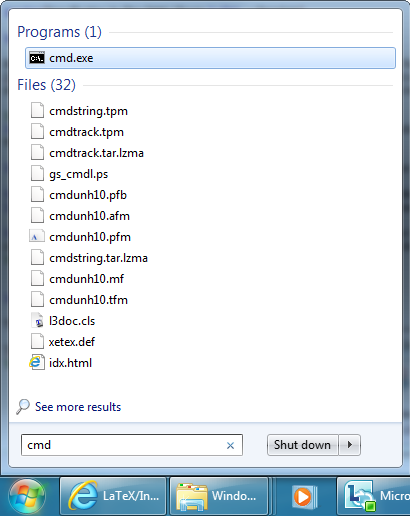
\includegraphics[width=\textwidth, height=0.4\textheight,keepaspectratio]{graphic/TAMUthesis_CMD_windows.png}
\caption{Open CMD (Command Line Interface) Under Windows}
[Open the data/chapterI.tex file to search for the implementation of this figure, as you can see that, to precisely contorl the position of the figure is not as straightforward as that in Office Word.]
\label{fig:CmdOpen}
\end{center}
\end{figure}

  
\begin{figure}[!htbp]
\begin{center}
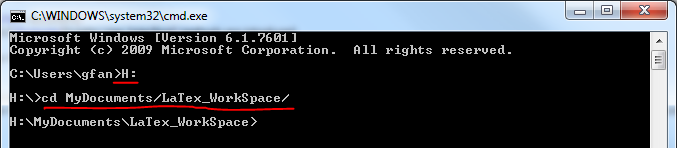
\includegraphics[width=\textwidth, height=0.4\textheight,keepaspectratio]{graphic/TAMUthesis_CMD_windows_cd.png}
\caption{Change Directory Command Under Windows}
[Before applying cd command in Windows, change to another disk segment by typing ``H:'' or ``D:'' instead of ``cd some\_path'']
\label{fig:CmdCd}
\end{center}
\end{figure}
  

\begin{figure}[!htbp]
\begin{center}
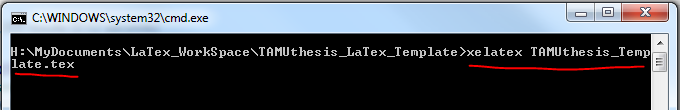
\includegraphics[width=\textwidth, height=0.4\textheight,keepaspectratio]{graphic/TAMUthesis_CMD_windows_compile.png}
\caption{Compile .tex File}
\label{fig:CompileLaTex}
\end{center}
\end{figure}
  
\begin{Contfigure}[!htbp]
\captionsetup{list=no}
\begin{center}
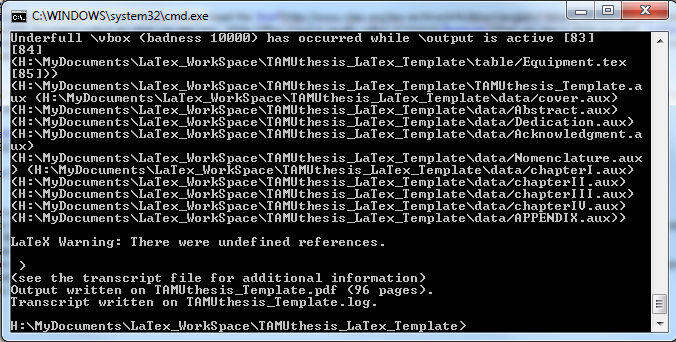
\includegraphics[width=\textwidth, height=0.4\textheight,keepaspectratio]{graphic/TAMUthesis_CMD_windows_compile2.png}
%\caption{Compile .tex File Output}
\caption{} %OGAPS thesis office requests the title of figure continued to have no text. All texts should appear under the main figures. I would suggest to just use fig 1.1, fig 1.2 etc for reference. Don't use continue figure. It's complex gaofeng@tamu.
\label{fig:CompileLaTex2}
[Example usage for Figure continued. Please Don't display text for Continued Figures. This is just an example.]
\end{center}
\end{Contfigure}  
  
  
\paragraph{GUI}
Open the .tex file using MikTeX and choose the option as shown in Figure \ref{fig:CompileLaTexGUI} to execute.

\begin{figure}[!htbp]
\begin{center}
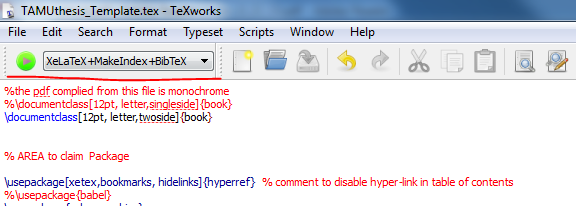
\includegraphics[width=\textwidth, height=0.4\textheight,keepaspectratio]{graphic/TAMUthesis_GUI_windows.png}
\caption{Compile .tex file Under Windows System}
\label{fig:CompileLaTexGUI}
\end{center}
\end{figure}

\subsection{How To Fill In This Document}
The document structure is organized in the main .tex file, TAMUthesis\_Template.tex, which has the same name as the output PDF file. Content in each chapter is under the folder of data. You can open the .tex files under the data folder to modify. Four chapters are added initially. To add in more chapters into the \LaTeX ~document, please open the TAMUthesis\_Template.tex files and goto line No. 280 as shown in Figure \ref{fig:AddChapter} .

\begin{figure}[!htbp]
\begin{center}
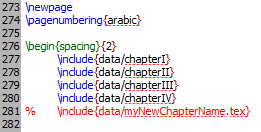
\includegraphics[width=\textwidth, height=0.3\textheight,keepaspectratio]{graphic/TAMUthesis_AddChapter.png}
\caption{Add More Chapters Into TAMUthesis\_Template.tex}
[For example, a new chapter named ``myNewChapterName.tex'' is created under the folder of \textbf{data}. To put this new file for the compilation by adding the line \verb|\include{data/myNewChapterName.tex}| as shown in 281 (uncomment the \% in front.).]
\label{fig:AddChapter}
\end{center}
\end{figure}

For the rest of the document, you can just delete the content in the data folder and fill your documents and then compile under TAMUthesis\_Template.tex.

\subsection{Reference Usage And Example}

This subsection test the usage of Reference. Paper\cite{AhmadiF} is referred in this way. Actually, the option is available for you to change the default way how reference appears. The default and most commonly used option \cite{PetterVary2006.March} is displayed here. Please download a free software called JabRef to manage your references. When you need any references, do search it on-line and download the bib format to import into the JabRef. 

Unrelated citations are referred here for test of Reference Section only\cite{Andraka1998}. If you find the Reference\cite{Azzarello2005} has more items than you need \cite{Beritelli2002}. It's possible that the old bbl file\cite{Boyd1985} is not updated yet.The simple solution\cite{Carew1998} is to delete the bll file and re-compile the whole PDF \cite{Callanan1995}. Of sometimes, if you really makes a mistake, read the .log files to see what is the error information there.

\subsection{Equation Usage}
It looks like there are some fundamental problems for \LaTeX~ to accurately control the vertical spacing above/below equations. While I have tried my best to fine tune the spaces above/below equations. You should pay special attentions when use two \textbf{equation} environments consecutively. As this might results in ugly large vertical spacing between equations and texts. As I have stated somewhere else in this document, I would suggest you to use \textbf{align} environment for a list of equations. And you can also refer and label them one by one as the example code shown in Equ. \eqref{x_cordic1}.

\subsection{Cover Page}
The default cover page has three line title which might not fit your case. The requirement for the cover page is not so strict. You can adjust the vertical space and find out the most balanced top/bottom margin for cover page. Hence, some fine tuning might be necessary from user perspective. Please refer to the \textbf{data} folder and open the file named cover.tex for modification.

\section{Specification In This TAMU Thesis \LaTeX  ~ Template}

\subsection{Chapter Method Requirement}

Below are the general requirements for thesis chapter from OGAPS. The bold/Italic font is applied to the setting that is currently implemented in this document when there is a choice\footnote{The default non-indentation setting is removed after reviewing with OGAPS. All the new paragraph will automatically indent. When writing the document in \LaTeX, just 'Enter' twice to leave a blank line for indentation. I see questions on-line about how to enable single space in footnote, the settings used in this \LaTeX~ document doesn't affect the single space setting in footnote, which is my lucky. So there is no local settings needed for footnote to keep in single space.}.

\begin{enumerate}
\item	Standard margins on this document is 1.4'' left, 1.15'' right, 1.25'' top and bottom. The page number (Arabic) 1 is outside the margin, at the bottom of the page and centered. Number every page of the thesis in sequence through the Appendix, which is the last page.

\item \textit{Chapter method} are mostly applied in organizing the document. Before the chapter method is stabilized/approved by OGAPS, no section method is going to be tested and verified.

\item the major heading consists of the chapter designation (CHAPTER I) and the title. Both are centered, in all capital letters. While chapter designation being in capital is automatically controlled by the \LaTeX ~, the title needs author to type in capital or use \LaTeX command \verb|\textsc{}| to brace the them. The effect of these two commands are a little bit difference but can all satisfy the thesis requirement.

\item if the \textit{chapter title} is longer than one line, use spacing of text between the lines of the title (\textbf{double space} or space-and-a-half). Use same front size as other major headings (\textbf{and bold if other major headings are bold}). Be consistent with spacing between chapter title and text for all chapters (one or two double spaces)
\end{enumerate}


\subsection{Subheadings Requirements}

This is the second-order subheadings in this \LaTeX ~ document.

TAMU graduate theses and dissertations do not have a specific "style" for subheadings.Some rules for ALL levels of subheadings are:
\begin{itemize}%[noitemsep, nolistsep]
	\item   Vertical spacing above and below each subheading needs to be consistent for \emph{each} level.
	\item   Vertical spacing within a subheading with more than one line needs to be the same as spacing of the text.
	\item   Include the chapter/major section number if numbering or lettering the subheadings, ex. I.1, II.1. or 1.1, 2.1 (first level subheadings) and I.1.1, II.1.1 or 1.1.1, 2.1.1 (second level subheadings)
	\item   Style and format need to match for \emph{each level} (numbering is enough to differentiate the levels -- if numbered they can look the same or each level can look different).
	\item   Type size and style need to follow text.
	\item  Capitalization needs to be consistent for \emph{each level} of subheading.
\end{itemize}

First-order subheadings, which are section in this \LaTeX ~ document, must be included in the Table of Contents, which is implemented in this TAMUthesis.

Second-order subheadings, which are subsections in this \LaTeX ~ document, need to differ from first level unless they are numbered. If numbered, all levels of subheadings may match for style (but they do not have to). Second levels do not need to be included in the Table of Contents.
\subsection{Third-Order Subheadings}
Third-order subheadings, if numbered, may match the other levels of subheadings. If unnumbered, they need to have a different style. Third levels do not need to be included  in the Table of Contents.


\section{Test Section}
Test Content is displayed below.

\section{Thesis Organization}
Example code below for \LaTeX ~ \textbf{description} environment.
\begin{description}
\item[The 1st chapter] introduces the background. 

\item[The 2nd chapter] briefly describes how to do it.

\item[The 3rd chapter] details the design of the hardware. Test and verification of this hardware is located in Appendix \ref{cha:appendix}.

\item[The 4th Chapter] issues the discussions and gives the summary. 

\item [The Appendix] contains some less-intersting, but still significant test benches, test setup details and test result information.  It is provided in Appendix \ref{cha:appendixB}. Appendix \ref{cha:appendixC} details the usage.
\end{description}
